\subsection{Panoramaerstellung}
\label{sec:Panoramaerstellung}

Die Panoramaerstellung stellt, neben der Softwareerstellung einen zentralen
Teilprozess innerhalb der Projektumsetzung dar. Innerhalb dieses Prozesses
werden die 360-Grad Panoramas, welche den eigentlichen Inhalt der Anwendung
darstellen, entworfen. Im Folgenden soll der Prozess der Panoramaerstellung
näher untersucht werden. Hierbei soll zunächst erläutert werden, in welcher
Form die Panoramafotos vorliegen müssen, um von der Anwendung verarbeitet
werden zu können. Weiterhin soll das Equipment vorgestellt werden, welches zur
Umsetzung der Panoramafotos benötigt wird. Anschließend soll dann der Workflow
der Panoramaerstellung dargestellt werden.

\subsubsection{Anforderungen an die Panoramafotos}
\label{sec:PanoramaerstellungAnforderungen}

Bevor mit der Erstellung der Panoramas begonnen werden kann müssen zunächst die
Anforderungen der Anwendung an die Panoramafotos festgelegt werden. Hierbei muss
definiert werden, welche Kriterien die Panoramafotos erfüllen müssen, um von der
Anwendung korrekt verarbeitet werden zu können. Relevante Kriterien sind hierbei
die Darstellungsform, die Größe und das Format der Panoramafotos. Nachdem diese
Schnittstelle festgelegt ist kann der Prozess der Panoramaerstellung isoliert
vom Prozess der Softwareerstellung durchgeführt werden. Dies ermöglicht eine
parallele Umsetzung der beiden Teilprozesse.

Wie bereits in \verweis{Architektur} erwähnt soll in der Anwendung die Google
Street View API verwendet werden. Diese Schnittstelle stellt die Funktionalität
zur Anzeige der Panoramafotos zur Verfügung. Somit legt diese Schnittstelle auch
fest, in welcher Form die Panoramafotos zur Verfügung gestellt werden müssen.
Diese Anforderungen können aus der Entwicklerdokumentation zu der API entnommen
werden. Die Schnittstelle erwartet hierbei ein Panoramafoto, welches der
Rektangulatprojektion\footnote{Die Rektangularprojektion stellt eine
horizontale Ansicht von 360 Grad und eine vertikale Ansicht von 180 Grad dar.
Dies bedingt ein Seitenverhälnis von 2:1} entspricht. Durch die API wird diese
Darstellung auf die Fläche einer Kugel projeziert. Der Mittlepunkt dieser Kugel
stellt den Standpunkt des Betrachters dar. Da sich immer nur ein Teil der
Projektion im Blickfeld dieses Betrachters befindet muss auch nur der aktuell
sichtbare Bereich des Panoramafotos dargestellt werden. Aus diesem Grund bietet
die Google Street View API die Möglichkeit, ein in mehrere rechteckige Teile,
sogenannte Kacheln, aufgeteiltes Panoramafoto zu verarbeiten. Auf diese Weise
kann die Performanz der Anwendung erhöht werden, da nicht das komplette
Panoramafoto, sondern nur ein Teil der Kacheln in der Anwendung geladen werden
muss. Damit den einzelnen Kacheln die korrekte Position auf der Planarprojektion
zugewiesen werden kann, muss die Benennung der Kacheldateien dem Namensschema
\texttt{Kachelspalte-Kachelzeile} genügen. Die Anzahl der Kacheln sowie die
Pixelmaße des Panoramafotos können frei gewählt werden. Hierbei ist zu beachten,
dass mit steigender Pixelanzahl die Qualität der 360-Grad-Darstellung steigt,
die Performance der Anwendung jedoch aufgrund der steigenden Datengröße sinkt.
In einer prototypischen Implementierung, auf die im \verweis{Softwareerstellung}
näher eingegangen werden soll, hat die Projektgruppe verschiedene Kombinationen
aus Pixekmaße und Kachelanzahl getestet. Letztendlich hat sich die Projektgruppe
auf die Pixelmaße 4096x2048 für das gesamte Panorama und eine Aufteilung in 8
mal 4 Kacheln entschieden. Diese Kombination wurde einheitlich als bester
Kompromiss zwischen Qualität und Performanz angesehen.

\subsubsection{Workflow der Panoramaerstellung}
\label{sec:Workflow}

Der Workflow der Panoramaerstellung kann mehrere Teilprozesse untergliedert
werden. Für die Umsetzung dieser einzelnen Teilschritte wird hierbei spezielles
Hard- und Softwareequipment benötigt. Im Folgenden sollen die einzelnen
Teilschritte der Panoramaerstellung in chronologischer Reihenfolge erläutert
werden. Hierbei soll auch auf das benötigte Equipment eingegangen werden.

\paragraph{Aufnahme der Einzelfotos} \hfill \\

Die Panoramaerstellung beginnt mit der Aufnahme mehrerer Einzelfotos. Aus diesen
Einzelfotos wird nachfolgend dann das komplette Panoramafoto zusammengefügt.
Dieses muss, wie zuvor erläutert, der Rektangularprojektion entsprechen. Die
Summe der Einzelfotos muss also eine horizontale Ansicht von 360 Grad und eine
vertikale Ansicht von 180 Grad abbilden. Die Anzahl der Einzelfotos ist somit
von dem Bildwinkel abhängig, der auf einem einzelnen Foto dargestellt werden
kann. Dieser Bildwinkel wird in der Fotografie durch die Brennweite des
Objektives festgelegt. Je geringer die Brennweite eines Objektives ist, desto
größer ist der Bildwinkel, der mit diesem Objektiv eingefangen werden kann und
desto Weniger Einzelfotos werden für die Panoramafotos benötigt. Durch
spezielle Objektivkonstruktionen wie zum Beispiel einem Fischaugenobjektiv ist
es möglich einen besonders großen Bildwinkel aufzunehmen. Ein solches Objektiv
und eine zum dem Objektiv kompatible Kamera wird auch für die Aufnahme der
Panoramafotos im Projekt verwendet. Das Objektiv ermöglicht es in 16 Fotos alle
Ansichten Aufzunehmen, die zur Darstellung einer Rektangularprojektion benötigt
werden. In 15 dieser Einzelfotos ist hierbei die horizontale Rundumansicht
dargestellt. Das sechzente Foto bildet den Zenit\footnote{Der Zenit ist der
Punkt über dem Beobachter/der Kamera} im Panoramafoto ab. Der
Nadir\footnote{Der Nadir ist der dem Zent gegenüber gelegene Punkt unter dem
Beobachter/der Kamera} wird in den Panoramafotos nicht abgebildet, da sich hier
das Stativ befindet. Die aufgenommenen Einzelfotos müssen sich überschneiden,
um ein späteres Zusammenfügen der Fotos zu ermöglichen.
% TODO: Kompass erwähnen?

Zur Unterstützung bei der Aufnahme hat sich die Projektgruppe weiterhin
entschieden ein speziell für die Panoramafotografie ausgelegtes Stativ zu
verwenden. Eine Aufnahme ohne dieses Stativ wäre zwar denkbar, würde die
Qualität der Panoramafotos jedoch stark beeinträchtigen. Dieses Panoramastativ
besteht aus folgenden Komponenten:

\begin{description}
\item[Stativ] Das eigentliche Stativ dient dazu, die Kamera im Raum an einer
festen Position zu fixieren. Hierdurch ist sichergestellt, dass alle
Einzelfotos von der selben Position aus aufgenommen werden.
\item[Nivelliervorrichtung] Die Nivelliervorrichtung dient dazu, den Kopf des
Statives horitontal auszurichten. Auf diese Weise wird ein wellenförmiger
Horizont in dem zusammengefügten Panoramafoto vermieden.
\item[Rotator] Der Rotator ermöglicht es, den Kopf des Stativs um die vertikale
Achse zu drehen. Weiterhin kann eine Gradzahl festgelegt werden, nachdem der
Machanismus bei einer Drehnung einrastet. Auf diese Weise wird eine gleichmäßige
Drehung bei der Aufnahme der Panoramafotos ermöglicht.
\item[Nodalpunktadapter] Der Nodalpunktadapter ermöglicht es, die Kamera auf
dem Stativ so zu positionieren, dass die Eintrittspupille des Stativs auf Höhe
der vertikalen Drehachse des Stativs liegt. Hierdurch können
Parallaxenfehler\footnote{Der Parallaxenfehler beschreibt eine scheinbare
Verschiebung zweier hintereinandergelegener Gegenstände, wenn sich der
Ausgangspunkt der Betrachtung ändert} bei der Aufnahme vermieden werden
\end{description}

Das komplette Equipment, welches zur Aufnahme der Panoramafotos verwendet wurde,
ist in \abbildung{Equipment} dargestellt.

\begin{figure}[htb]
\centering
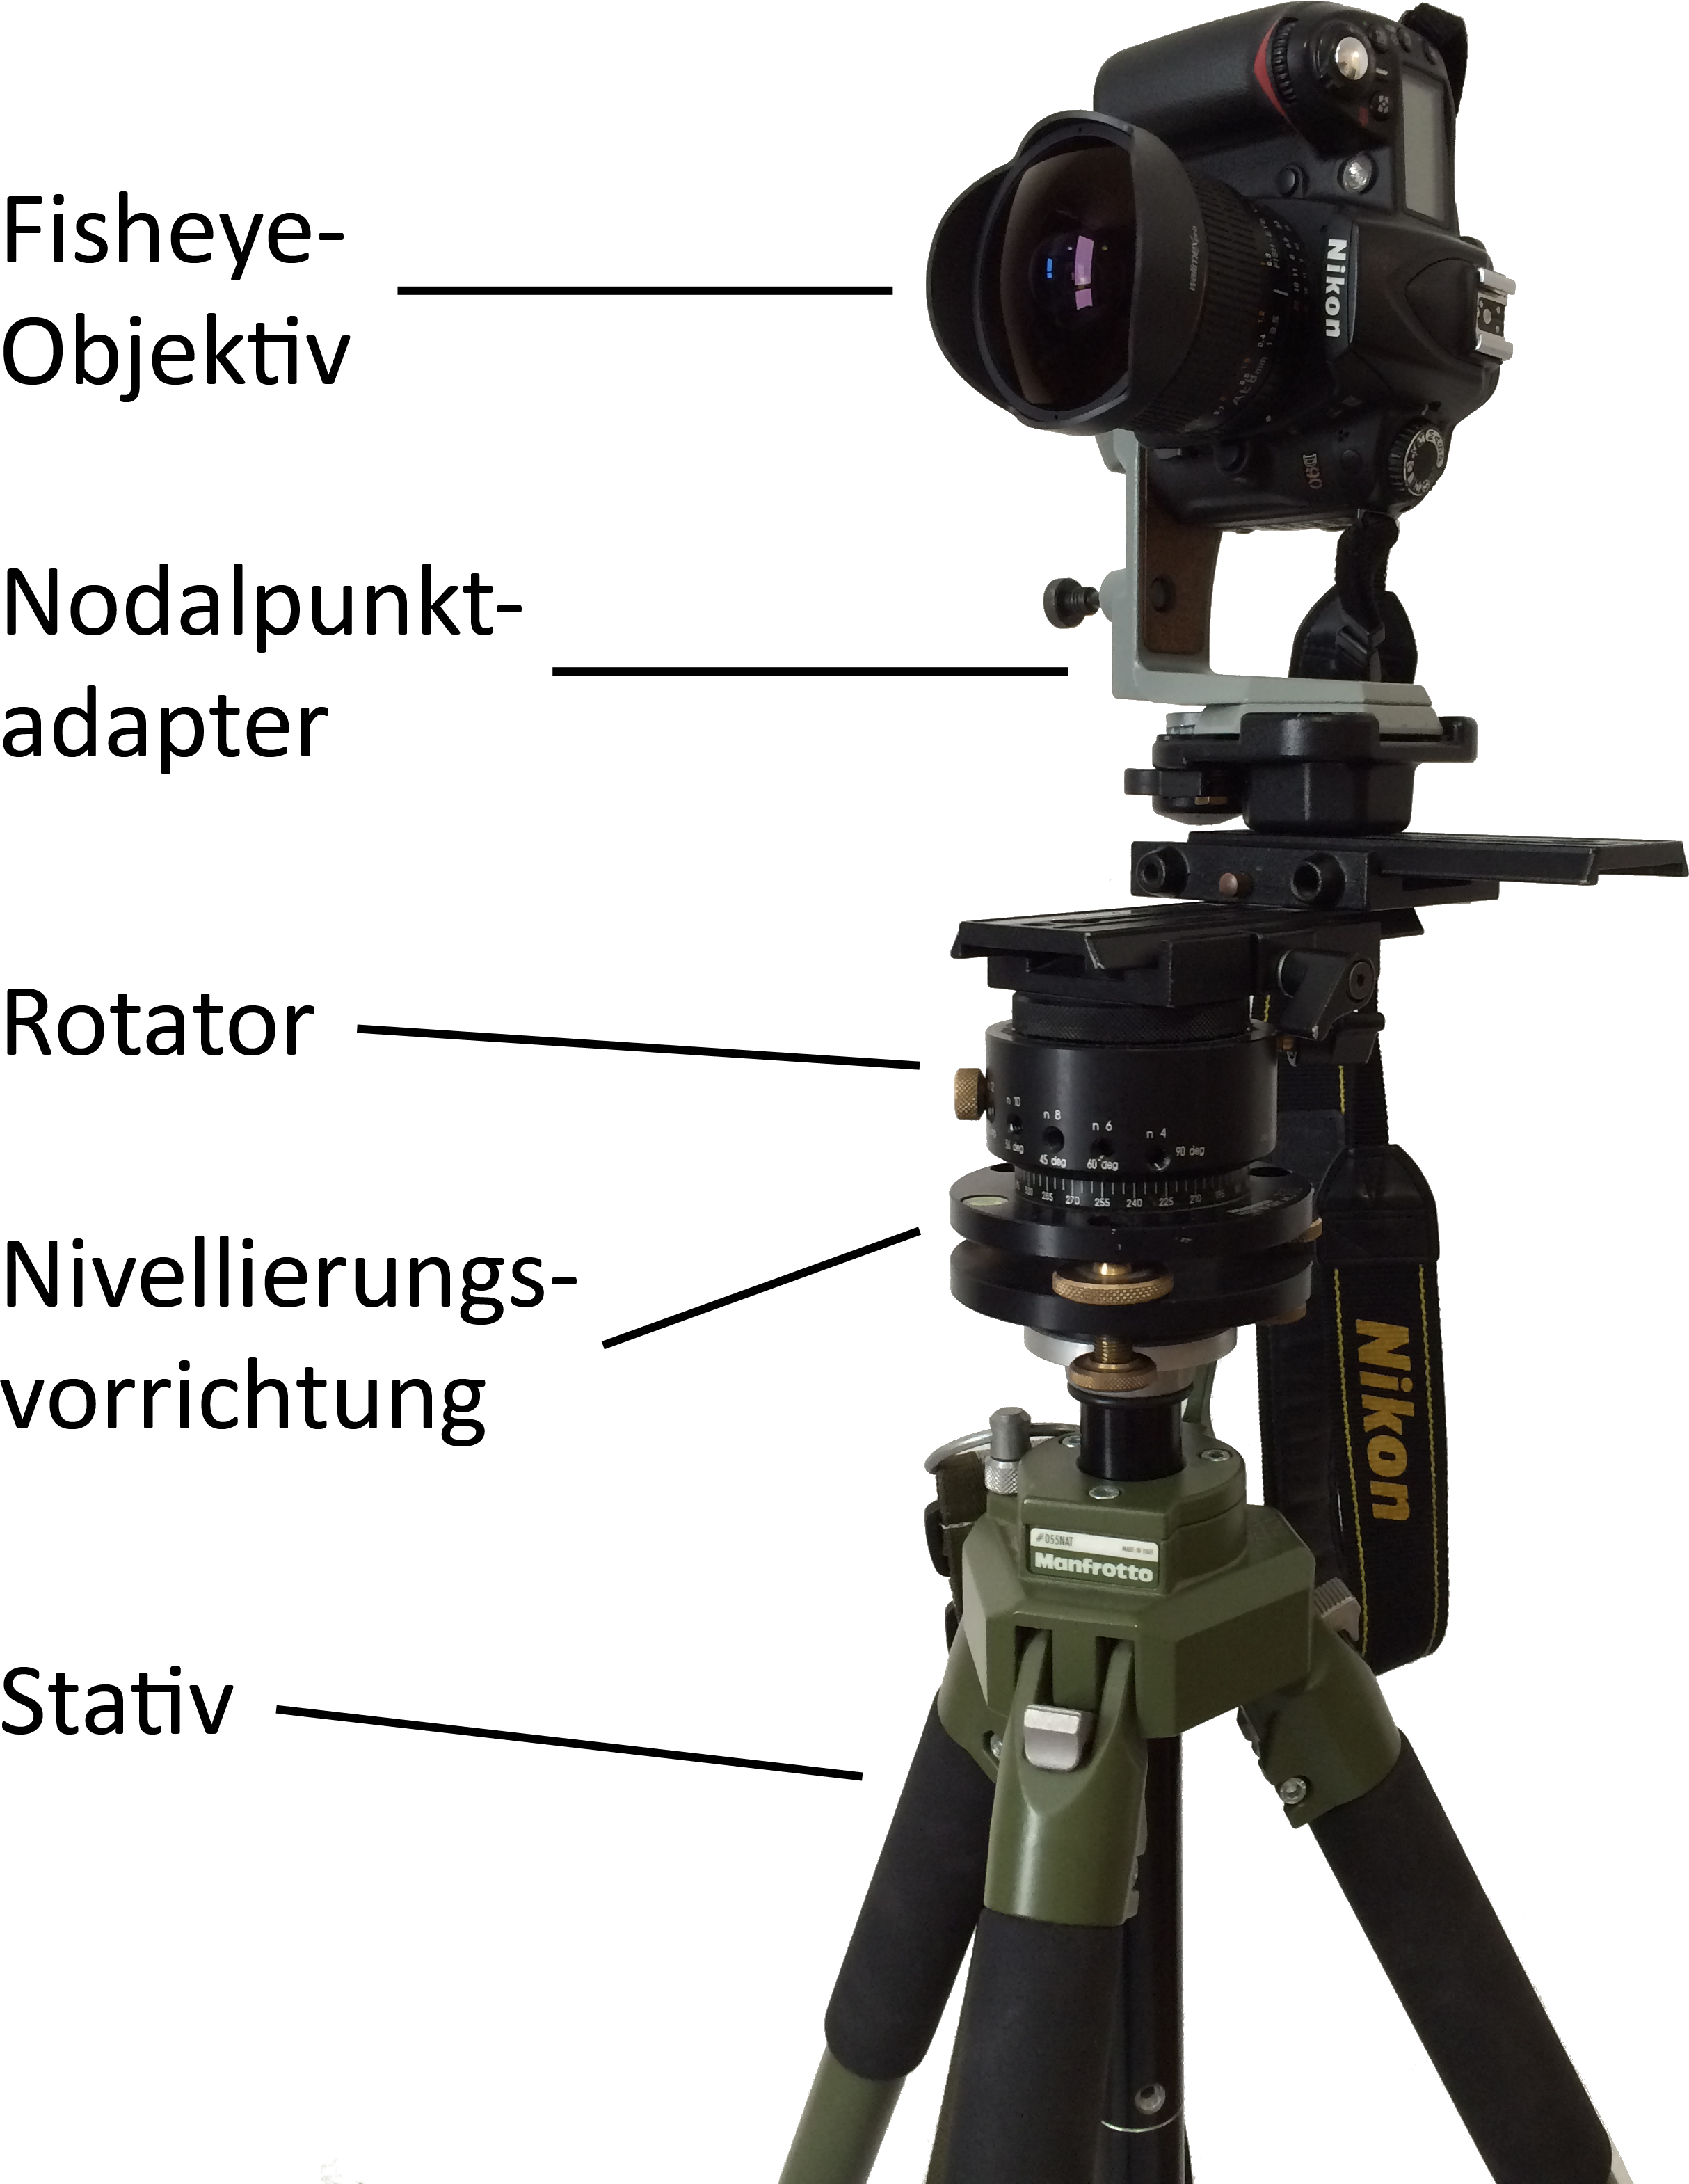
\includegraphics[width=0.5\textwidth]{Equipment.png}
\caption[Equipment zur Aufnahme der Einzelfotos]{Equipment zur Aufnahme der Einzelfotos\protect\footnotemark}
\label{fig:Equipment}
\end{figure}
\footnotetext{Eigene Darstellung}

\paragraph{Stitching und Rendering} \hfill \\

Nachdem die Einzelfotos aufgenommen wurden müssen diese zu einem Panoramafoto
zusammengefügt werden. Dieser Prozess wird als Stitching bezeichnet. Das
Stitching erfolgt im Projekt mit der Software Kolor Autopano Giga 3.0. Die
Software ist in der Lage die Einzelfotos automatisiert Zusammenzufügen.
Gegebenenfall muss das hieraus resultierende Panoramafoto nach dem
automatisierten Zusammenfügen noch manuell ausgerichtet werden. Aufgrund
dieser manuellen Ausrichtung ist es nicht möglich den hier beschriebenen
Prozess vollständig zu automatisieren. In einem letzen Schritt wird das
zusammengefügte Panoramafoto dann in das JPEG-Format konvertiert. Dieser Schritt
wird als Rendering bezeichnet. Das Ergebnis dieses Prozesses ist in Abbildung X
% TODO: Abbildung einfügen
dargestellt.

\paragraph{Abschließende Bearbeitung} \hfill \\

Wie bereits zvor beschrieben war es bei der Aufnahme der Einzelfotos nicht
moglich den Nadir Abzubilden, da sich dort das KAmerastativ befand. Diese
Bildinformationen fehlen folglich auch in dem zusammengefügten Panoramafoto. Der
Bereich, in dem Bildinformationen fehlen, ist in Abbildung X
%TODO: Abbildung einfügen
durch eine schwarze Fläche markiert.

In einer abschließenden Bearbeitung\ldots

\ldots Die Komplette Bearbeitung erfolgt mit der Software Adobe Photoshop CS5
